\documentclass[11pt,a4paper]{article}
\usepackage[margin=23mm]{geometry}
\usepackage{amsmath,amssymb,fontspec,unicode-math,lmodern}
\setmainfont{texgyrepagella-regular.otf}[BoldFont=texgyrepagella-bold.otf,ItalicFont=texgyrepagella-italic.otf,BoldItalicFont=texgyrepagella-bolditalic.otf]
\setmathfont{texgyrepagella-math.otf}
\setmonofont{lmmono10-regular.otf}
\usepackage{amsmath,booktabs,array,graphicx,xcolor,hyperref,xurl,fancyhdr}
\definecolor{inkblue}{HTML}{176B91}
\hypersetup{colorlinks=true,linkcolor=inkblue,citecolor=inkblue,urlcolor=inkblue,pdftitle={Paper G: Geometry-Attached Axial Observables},pdfauthor={Hilmir Frímann Halldórsson}}
\graphicspath{{../figures/}}
\pagestyle{fancy}\fancyhf{}\fancyhead[L]{\small Paper G v0.1.1}\fancyhead[R]{\small LOCAL REVIEW DRAFT}\fancyfoot[C]{\thepage}
\setlength{\headheight}{14pt}\setlength{\parskip}{4pt}\setlength{\parindent}{0pt}
\setlength{\emergencystretch}{2em}
\raggedbottom\clubpenalty=10000\widowpenalty=10000\displaywidowpenalty=10000
\newtheorem{theorem}{Theorem}\newtheorem{proposition}[theorem]{Proposition}\newtheorem{lemma}[theorem]{Lemma}
\newenvironment{proof}{\par\textit{Proof.}\ }{\hfill$\square$\par}
\newcommand{\R}{\mathbb R}\newcommand{\C}{\mathbb C}\newcommand{\Om}{\Omega}\newcommand{\Fh}{\widehat F}\newcommand{\cof}{\operatorname{cof}}\newcommand{\diag}{\operatorname{diag}}\newcommand{\Argz}{\operatorname{Arg}_0}\newcommand{\iu}{\mathrm i}\newcommand{\dd}{\mathrm d}
\title{\vspace{-10mm}Geometry-Attached Axial Observables,\newline Period-Doubling, and Certified Entrance Capture\newline in the Tri-Octagon Map}
\author{Hilmir Frímann Halldórsson}
\date{Paper G v0.1.1 \quad 4 October 2026\\\small LOCAL REVIEW DRAFT: prepared for author and scientific review}
\begin{document}
\maketitle\thispagestyle{fancy}
\begin{abstract}
The three-channel complex map of Paper A admits signed channel areas but those areas are not themselves an ambient axial vector. Using the oriented tangent frames of Paper B, we construct the planar axial observable $W=TC$ from $C=\operatorname{Re}\Om\times\operatorname{Im}\Om$ and retain the complementary scalar $\Gamma=e^TC$. We prove the reconstruction and real-linear uniqueness statements, derive exact finite-step source accounting, and show how unequal amplitude coefficients expose an initially hidden Fourier-entrance area in $W$. The zero-area assertion is conditional: the adopted zero-component phase convention has an explicit exception. For a specified unequal-coefficient model, an outward interval certificate establishes a positive cubic flip coefficient and hence a local attracting family of alternating two-cycles. Separately, at the exact critical phase strength plus $1/200$, a repaired five-dimensional interval certificate proves that the normalized Fourier entrance reaches a trapping box at update 301. Two-step contraction and a separate symmetry-existence certificate yield a full complex two-cycle; a summability argument lifts the approaching quotient trajectory to one constant rotation of that cycle. The local bifurcation and the fixed-parameter capture are not joined by a proved continuation. Exact identities, computer-assisted theorems and finite numerical illustrations are distinguished throughout. These are mathematical statements about a specified discrete map, not physical validation of magnetism.
\end{abstract}
\textbf{Status and scope.} This is a local review manuscript, not externally peer reviewed, published or assigned a DOI. Internal M1--M3 acceptance identifies the mathematical premises; it is not journal acceptance. No magnetic units, Maxwell law, material motion, calibrated energy or dynamo interpretation is adopted.

\section{Problem, model and evidence}
The question is whether a geometrically meaningful axial observable can be extracted from the already defined dynamics, and whether that observable can persist along an orbit reached from a specified entrance. Three logically different answers are needed. A kinematic construction attaches signed channel areas to fixed geometry. A local bifurcation theorem establishes an alternating branch near a real host. A finite entrance certificate establishes capture by a two-cycle at a particular parameter. None of these steps substitutes a visual pattern for a theorem.

We use the map of Paper A \cite{PA}, the outward-oriented frames and transported area convention of Paper B \cite{PB}, and the corrected, jointly accepted M1, M2 and M3 source records \cite{M1,M2,M3}. Paper E's staged and committed-EMA readouts remain distinct observables \cite{PE}; neither is $W$. Paper F provides limited local angular background, not a continuation result for the unequal-coefficient model here \cite{PF}. Atlas 08 supplies the already adopted Fourier-form endpoint context \cite{Atlas}; its preparation and physical interpretation are not prerequisites of the present theorems.

We distinguish \emph{exact algebraic deductions}, \emph{computer-assisted theorems} based on outward enclosures, and \emph{nominal numerical illustrations}. The latter cannot upgrade an unproved parameter range or a rounded experiment to an exact-model theorem. The accompanying claim map identifies the final corrected sources for each statement. Standard flip, contraction and interval-existence methods are used with attribution; no global novelty claim is made.

\subsection{State space and ordered update}
Let $\Om=(\Om_A,\Om_B,\Om_C)^T\in\C^3$, $e=(1,1,1)^T$ and $L=ee^T-3I$. All parameters $\epsilon,g,\lambda,k_A,k_B,k_C$ are real. Define the amplitude map $\mathcal A$ and then the simultaneous phase map by
\begin{align}
 \widetilde\Om_i=\mathcal A(\Om)_i
 &=\Om_i+\epsilon\Om_i(k_i-|\Om_i|^2)+g(L\Om)_i,\label{eq:amp}\\
 \phi_i&=\Argz(\widetilde\Om_i),\qquad
 \delta_i=\lambda\sum_{j\ne i}\sin\bigl(3(\phi_j-\phi_i)\bigr),\label{eq:phase}\\
 F_\lambda(\Om)_i=\Om_i^+
 &=|\widetilde\Om_i|\exp\bigl(\iu(\phi_i+\delta_i)\bigr).\label{eq:full}
\end{align}
Here $\Argz(0)=0$; away from zero it is the principal argument, with its branch immaterial to the displayed exponentials and integer harmonics. All $\delta_i$ use the same pre-sync state. The update is not sequential in the channels. The graph Laplacian has eigenvalues $0,-3,-3$. No conservation of total intensity is assumed.

On the open set where every pre-sync component is nonzero, $F$ is smooth and common-phase equivariant. Its amplitude part is a cubic nonlinear map: the representation $\mathcal A(\Om)=M(\Om)\Om$ has a real, \emph{state-dependent} matrix, not a fixed linear operator. Conjugation equivariance holds with the stated phase convention. Permutation covariance carries $k$ with the labels. Fixed unequal $k$ is not generally invariant under all channel permutations.

\begin{table}[ht]
\centering\small
\begin{tabular}{p{.19\linewidth}p{.74\linewidth}}\toprule
Symbol & Meaning and space\\\midrule
$S,A$ & Symmetric Gram part and antisymmetric area matrix, real $3\times3$.\\
$C,W,\Gamma$ & Channel area vector, ambient planar axial vector, complementary signed scalar.\\
$\mathcal A,M$ & Nonlinear amplitude map and its state-dependent real matrix.\\
$J,\mathcal B,\mathcal C$ & Quotient Jacobian and its second/third derivative tensors at the host.\\
$T,T_{ij}$ & Tangent-column attachment matrix and matched tangent-plane transport.\\
$H_s,H$ & Spatial horizontal reflection and its conjugation action in quotient coordinates.\\
$V$ & Orthonormal basis matrix of $u^\perp$, not the spatial mirror.\\
$c_{\rm nf},c_*,r_i$ & Flip coefficient, trap center, positive trap weights.\\
$\Om_*^{(+)},\Om_*^{(-)}$ & Full complex cycle states in M2 or M3, scoped to each theorem.\\\bottomrule
\end{tabular}
\caption{Notation keeps channel area, evolution, geometry and proof coordinates distinct.}
\end{table}

\section{From transported area to an axial observable}
\subsection{Areas and the Paper B attachment}
Writing $\Om=x+\iu y$ with $x,y\in\R^3$, set
\begin{equation}
 S=xx^T+yy^T,\quad A=xy^T-yx^T,\quad
 C=x\times y=(A_{BC},A_{CA},A_{AB})^T.\label{eq:SA}
\end{equation}
Thus $A=-[C]_\times$, $\Om\Om^\dagger=S-\iu A$, while $\overline\Om\Om^T=S+\iu A$. The sign distinction matters in phase transport. Paper B identifies $A_{ij}$ with the signed parallelogram area of two face-state vectors after the matched transport $T_{ij}=t_it_j^T+e_ze_z^T$. No factor $1/2$ occurs.

The fixed outward normals and horizontal tangents are
\begin{equation}
 N=\begin{pmatrix}-\sqrt3/2&0&\sqrt3/2\\1/2&-1&1/2\\0&0&0\end{pmatrix},\quad
 T=\begin{pmatrix}-1/2&1&-1/2\\-\sqrt3/2&0&\sqrt3/2\\0&0&0\end{pmatrix},\label{eq:T}
\end{equation}
whose columns are $n_i$ and $t_i=e_z\times n_i$. The actual face centers are $(-1/4,\sqrt3/4,0)$, $(0,0,0)$ and $(1/4,\sqrt3/4,0)$. A complex entry is encoded as the tangent vector $x_it_i+y_ie_z$. The panels are fixed; the encoding adds no material dynamics. Define
\begin{equation}
 W=TC,\qquad \Gamma=e^TC,\qquad
 C_\parallel=\frac{\Gamma}{3}e,\quad C_\perp=C-C_\parallel.\label{eq:W}
\end{equation}
These have the algebraic scale of squared state amplitude, not tesla or another physical unit. The orientation of $C$ lives in channel space. Equation \eqref{eq:W} is the specified map from that space into the ambient geometry.

\begin{proposition}[Attachment, reconstruction and symmetry]\label{prop:attach}
The attachment has rank two, kernel $\R e$, and
\begin{equation}
 T^TT=\frac32\left(I-\frac{ee^T}{3}\right),\qquad
 C=\frac23T^TW+\frac{\Gamma}{3}e,\qquad
 |C|^2=\frac23|W|^2+\frac{\Gamma^2}{3}.\label{eq:reconstruct}
\end{equation}
Under the specified $D_{3h}$ geometry action, $W$ is an ambient axial vector. Up to a real scalar, $T$ is the only real-linear equivariant map from this representation of $C$ to an ambient axial vector.
\end{proposition}
\begin{proof}
The three columns of $T$ sum to zero and have mutual inner products $-1/2$; their squared lengths are one. This proves the matrix identity and rank. Applying it to $C_\perp$ gives reconstruction; orthogonality gives the norm identity.

For a spatial orthogonal symmetry $G$ with channel permutation $Q$, Paper B's area action is $A'=\det(G)QAQ^T$, so
\begin{equation}
 C'=\det(G)\det(Q)QC.\label{eq:Ccov}
\end{equation}
The frame matrices obey $T\det(Q)Q=GT$, verified on the cyclic rotation, horizontal mirror $H_s=\diag(1,1,-1)$ and vertical mirror $V_s=\diag(-1,1,1)$ (which swaps the channel labels $A$ and $C$). Consequently $W'=\det(G)GW$. In contrast $\Gamma$ has generator signs $(+,-,+)$; $\Gamma e_z$ is polar-$z$-like, not axial. The distinct transformation laws forbid replacing $T$ by $N$.

For uniqueness, horizontal reflection acts as $-I$ on $C$ but as $\diag(-1,-1,1)$ on an axial vector. An intertwiner therefore has zero $z$ row. The invariant input line $\R e$ has no nonzero image in the planar cyclic representation. On $e^\perp$, $T$ identifies the two real planar representations. An endomorphism commuting with a $120^\circ$ rotation has the form $aI+bJ_2$; commuting also with the vertical mirror forces $b=0$. Hence the intertwiner is a scalar multiple of $T$.
\end{proof}

This uniqueness is explicitly restricted to real-linear functions of $C$. It is not a catalogue of nonlinear covariants. For example, with $p=(S_{AA},S_{BB},S_{CC})$ and $r=(S_{BC},S_{CA},S_{AB})$, M1's $K_4=e\cdot(p\times r)$ gives a conjugation-even axial-$z$ covariant $K_4e_z$. At $\Om=(1,2,3)$, $C=0$ but $K_4=12$. Neither this covariant nor complex conjugation acquires a physical field or time-reversal interpretation here.

\begin{figure}[htbp]\centering
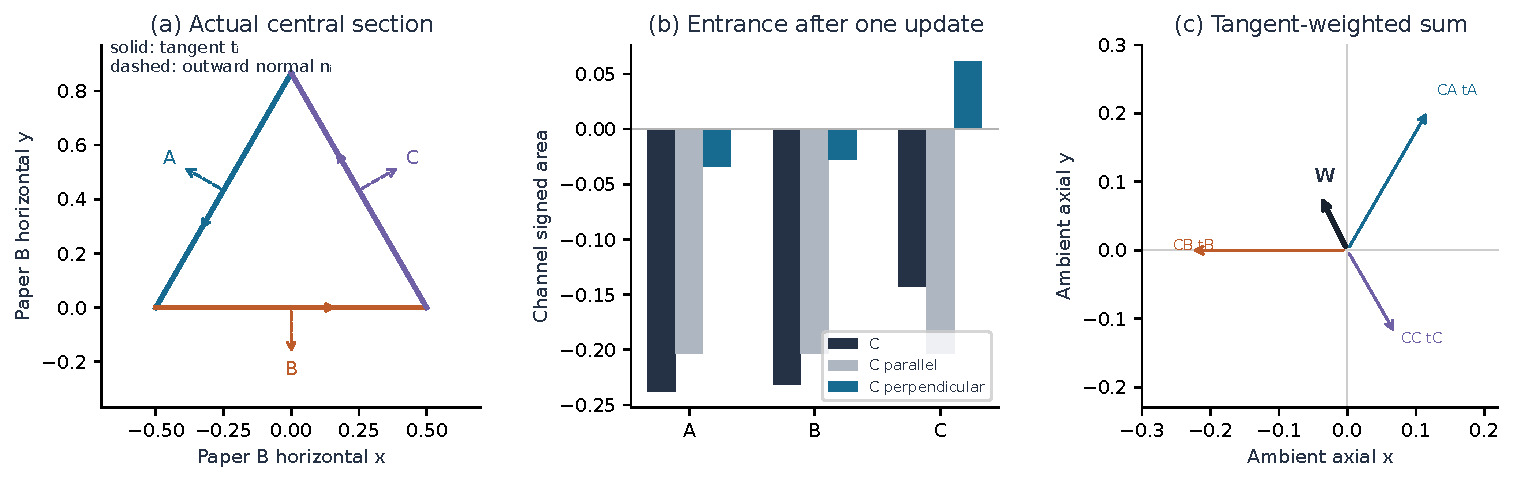
\includegraphics[width=\linewidth]{01_geometry_observable.pdf}
\caption{Paper B's actual central-section geometry and the M1 attachment. Panel (a) uses the fixed centers and unit-frame directions with a common display scale. Panels (b,c) use the correctly normalized M3 entrance after one nominal update. The channel decomposition and the tangent-weighted sum are different coordinate spaces. Arrow anchoring in (c) is a free-vector display convention; no spatial field or flux is drawn.}
\label{fig:geometry}\end{figure}

\subsection{Accounting identities}
Let $I_\Omega=\operatorname{tr}S=\|\Om\|^2$. Direct expansion of the Gram matrix gives
\begin{equation}
 SC=0,\quad e_2(S)=|C|^2,\quad
 I_\Omega^2=|\Om\cdot\Om|^2+4|C|^2,\quad |C|\le I_\Omega/2.\label{eq:gram}
\end{equation}
Here $e_2$ is the sum of principal $2\times2$ minors and $\Om\cdot\Om$ is bilinear, without conjugation. The identity follows also from $|x\times y|^2=|x|^2|y|^2-(x\cdot y)^2$. Area vanishes exactly when $x,y$ are linearly dependent, equivalently $\Om=cr$ for a complex scalar $c$ and a real vector $r$. However, $W=0$ only requires $C$ to be parallel to $e$; nonzero hidden area can remain in $\Gamma$.

\section{Exact finite-step source and entrance conversion}
\subsection{Amplitude congruence and phase-pair rotation}
For the current state define $D=\diag(k_i-|\Om_i|^2)$ and $M=I+\epsilon D+gL$. Since $M$ is real,
\begin{equation}
 \widetilde S=MSM^T,\qquad\widetilde A=MAM^T,\qquad
 \widetilde C=\cof(M)C.\label{eq:cof}
\end{equation}
The cross-product identity is polynomial in the entries of $M$. Thus it remains valid at singular $M$; an inverse formula is unnecessary. Although $M$ acts linearly on the two supplied vectors during this evaluation, its dependence on their intensities makes the underlying amplitude map nonlinear.

Expanding the congruence, using symmetric $D,L$, yields the exact budget
\begin{align}
 \widetilde A-A={}&\epsilon(DA+AD)+g(LA+AL)+\epsilon^2DAD\nonumber\\
 &+\epsilon g(DAL+LAD)+g^2LAL.\label{eq:budget}
\end{align}
The mixed and squared terms are finite-step contributions. Omitting them is a small-step approximation, not an alternative exact source law. Each term has a corresponding $C$ triple, $W$ vector and $\Gamma$ scalar by the fixed linear maps in \eqref{eq:SA} and \eqref{eq:W}.

For $d_{ij}=\delta_j-\delta_i$, complex multiplication of the pair product gives
\begin{align}
 A_{ij}^+&=\widetilde A_{ij}\cos d_{ij}+\widetilde S_{ij}\sin d_{ij},\label{eq:rotateA}\\
 S_{ij}^+&=\widetilde S_{ij}\cos d_{ij}-\widetilde A_{ij}\sin d_{ij}.\label{eq:rotateS}
\end{align}
Hence the phase contribution to $\Delta A_{ij}$ is precisely
$\widetilde A_{ij}(\cos d_{ij}-1)+\widetilde S_{ij}\sin d_{ij}$. These are entrywise trigonometric products; they are not matrix sine or cosine. The definition via \eqref{eq:phase} is valid at zero components too. Phase synchronization preserves each post-amplitude modulus but need not preserve the area vector.

\subsection{The Fourier entrance has hidden area}
Let
\begin{equation}
 (f_j)_n=3^{-1/2}e^{-2\pi\iu jn/3},\qquad n=0,1,2,\quad j=1,2.
\end{equation}
For $\Om=cf_j$ and $Q=|c|^2$,
\begin{equation}
 C(cf_1)=-\frac{\sqrt3 Q}{6}e,\quad
 C(cf_2)=+\frac{\sqrt3 Q}{6}e,\qquad W(cf_j)=0.\label{eq:hidden}
\end{equation}
Since $L\Om=-3\Om$ and $|\Om_i|^2=Q/3$, put
\begin{equation}
 b_i=1+\epsilon(k_i-Q/3)-3g.
\end{equation}
Then $\widetilde\Om_i=b_i\Om_i$ and, with $C_0$ the common initial channel area,
\begin{equation}
 \widetilde C=C_0(b_Bb_C,b_Cb_A,b_Ab_B)^T.\label{eq:entrance}
\end{equation}
When all $b_i\ne0$, sign changes only add $\pi$ to component phases. All phase differences remain multiples of $\pi/3$, so every harmonic-three torque vanishes exactly and $C^+=\widetilde C$.

\begin{proposition}[One-step exposure of entrance area]
If $c\ne0$, $\epsilon\ne0$ and every $b_i\ne0$, then $W^+\ne0$ if and only if $k$ is not uniform.
\end{proposition}
\begin{proof}
By Proposition \ref{prop:attach}, $W^+=0$ exactly when the three pair products in \eqref{eq:entrance} agree. Dividing by their nonzero factors forces $b_A=b_B=b_C$, equivalently $k_A=k_B=k_C$. Conversely uniform $k$ gives a uniform area triple.
\end{proof}
This is conversion of an existing area into the observable plane. It is not generation of total area from a zero-area state. No claim passes through a vanishing $b_i$ by continuity of the missing phase. Nor does one nonzero output prove long-term persistence.

\subsection{Zero-component exception and the limits of closure}
If $A=0$, the real amplitude congruence preserves zero area. Write a nonzero pre-sync state as $\widetilde\Om=e^{\iu\alpha}r$ with $r$ real, absorbing the scalar magnitude in $r$. If every $r_i\ne0$, differences are $0$ or $\pi$, so phase torques vanish. Thus zero area is preserved in the nonzero pre-sync domain (and also when $\lambda=0$). The all-zero state is fixed.

If exactly one component $r_i=0$, the assigned phase there is zero instead of the common-phase continuation. For cyclic $(i,j,k)$ the exact remaining area is
\begin{equation}
 A_{jk}^+=r_jr_k\sin\!\left(\lambda[\operatorname{sgn}r_j-\operatorname{sgn}r_k]\sin3\alpha\right),\quad
 C^+=A_{jk}^+e_i.\label{eq:zeroexception}
\end{equation}
For opposite signs, nonzero $\lambda$ and nonzero $\sin3\alpha$ do not suffice: the sine can vanish at resonance. For example, $\lambda=\pi/2$, $\alpha=\pi/6$ gives zero. As a genuine exception to universal invariance, take $\Om=e^{\iu\pi/6}(1,-1,0)$, $\epsilon=g=0$ and $\lambda=\pi/12$. Then $A=0$ but
\begin{equation}
 A_{AB}^+=-1/2,\quad C^+=(0,0,-1/2),\quad W^+=(1/4,-\sqrt3/4,0).
\end{equation}
The same zero-stratum mechanism occurs with nonzero amplitude and coupling: at $\epsilon=1/20$, $g=1/5$, $k=e$ and $\lambda=1/1000$, this state gives $A_{AB}^+=-(4/25)\sin(1/500)$. These statements retain $\Argz(0)=0$ rather than silently regularizing it.

On the positive-intensity pre-sync domain, $G_c=S+\iu A$ supports a closed pair representation: let $q_{ij}=\widetilde G_{c,ij}/\sqrt{\widetilde G_{c,ii}\widetilde G_{c,jj}}$, compute $\delta_i=\lambda\sum_{j\ne i}\operatorname{Im}(q_{ij}^3)$ and set $G_{c,ij}^+=\widetilde G_{c,ij}e^{\iu d_{ij}}$. This formula divides by nonzero intensities. It is not a global Gram closure through the exceptional stratum. $A$ alone is not closed even away from that stratum: the states $(1,\iu,1)$ and $(2,\iu/2,2)$ have the same $A$, but at $\epsilon=1/10$, $k=e$, $g=\lambda=0$ their output area factors are respectively $1$ and $301/400$.

\section{A certified local supercritical flip}
\subsection{Exact parameters, host and quotient}
From here through the capture theorem, fix
\begin{equation}
 \epsilon=\frac1{20},\quad g=\frac15,\quad
 k=(1,1.2208964704604097,6.35310346037241).\label{eq:params}
\end{equation}
The displayed terminating decimals are exact rationals. Let $u$ be the unique positive root in the M2 certified host box of
\begin{equation}
 \epsilon u\odot(k-u^2)+gLu=0.
\end{equation}
Its approximate coordinates are $(1.554467816928818,1.573421131869043,2.085939972794636)$. Existence and uniqueness come from strict Krawczyk inclusion, not from this decimal display or a small Newton residual. The supplement gives the exact dyadic box, chosen center and enclosing image.

Set $a_{12}=\sqrt{u_A^2+u_B^2}$, $r_u=\|u\|$, and define
\begin{equation}
 v_1=\frac{(u_B,-u_A,0)^T}{a_{12}},\quad
 v_2=\frac{(u_Au_C,u_Bu_C,-a_{12}^2)^T}{a_{12}r_u},\quad V=(v_1\ v_2).
\end{equation}
Then $V^TV=I_2$ and $V^Tu=0$. Use the slice
\begin{equation}
 s(z)=u+\xi+\iu V\eta,\quad z=(\xi,\eta)\in\R^3\times\R^2,\qquad u^T(u+\xi)>0.
\end{equation}
For $u^T\Psi\ne0$, rotate $\Psi$ by $e^{-\iu\arg(u^T\Psi)}$ and read its slice coordinates using $V^T$; call this operation $\mathcal Q$. The quotient map is $\Fh_\lambda=\mathcal Q\circ F_\lambda\circ s$. We only use charts with nonzero pre-sync entries and nonzero gauge denominator. Conjugation is $H(\xi,\eta)=(\xi,-\eta)$. The observables $C,W,\Gamma$ are unchanged by a common-phase rotation and odd under conjugation.

\subsection{Exact compression and the crossing}
Write $M_u=I+\epsilon\diag(k-u^2)+gL$. At the positive real host the full real and imaginary blocks are
\begin{equation}
 J_R=M_u-2\epsilon\diag(u^2),\quad
 J_I=\diag(u)(I+3\lambda L)\diag(u)^{-1}M_u.\label{eq:linear}
\end{equation}
The phase direction has multiplier one. Quotienting removes that direction. Using
\[\diag(u)L\diag(u)^{-1}=u(1/u)^T-3I,\qquad V^Tu=0,\]
we obtain
\begin{equation}
 B(\lambda)=V^TJ_IV=(1-9\lambda)V^TM_uV.\label{eq:compression}
\end{equation}
Let $m_1>m_2$ be the eigenvalues of the symmetric compression $V^TM_uV$. M2's interval chain verifies $0<m_2<m_1<1$, with displays
\begin{equation}
 m_1\simeq0.4334093508963767,\quad m_2\simeq0.3331321545361646.
\end{equation}
Consequently
\begin{equation}
 \lambda_c=\frac{1+1/m_1}{9}\simeq0.36747639460421353655,\qquad \sigma=9m_1>0.\label{eq:critical}
\end{equation}
At $\lambda_c$ the critical multiplier is simply $-1$ with derivative $-\sigma$. The other imaginary multiplier is $-m_2/m_1\simeq-0.7686316731$. Positive leading principal minors of $J_R$ and $0.7I-J_R$ enclose its spectrum in $(0,0.7)$. The simple crossing is therefore isolated from all other quotient multipliers. The equal-$k$ double crossing is a different problem and is not covered by this argument.

\subsection{The cubic coefficient includes amplitude slaving}
At criticality write
\begin{equation}
 \Fh(z)=Jz+\tfrac12\mathcal B(z,z)+\tfrac16\mathcal C(z,z,z)+O(\|z\|^4).
\end{equation}
Use real right and left eigenvectors $Jq=-q$, $J^Tp=-p$, $\|q\|=1$, $p^Tq=1$. They occupy the imaginary block, where the symmetric compression allows $p=q$. The $H$-even vector $\mathcal B(q,q)$ occupies the real block. With $p^Tw=0$, the center embedding and coefficient convention are
\begin{align}
 z(a)&=aq+\tfrac12a^2w+O(a^3),\quad w=(I-J)^{-1}\mathcal B(q,q),\\
 c_{\rm nf}&=\tfrac16p^T\mathcal C(q,q,q)+\tfrac12p^T\mathcal B(q,w).\label{eq:cnf}
\end{align}
The quadratic invariance equation gives $(I-J)w=\mathcal B(q,q)$. The projected cubic embedding correction cancels because $p^TJ=-p^T$. This explains why the coefficient is the flip coefficient of the full quotient map, rather than a phase-only cubic term. Its numerical split is
\begin{equation}
 c_{\rm nf}\simeq0.2353870304413968-0.1488621807196093
 =0.08652484972178754.
\end{equation}
The negative slaved contribution is substantial. It cannot be discarded without changing the normal form.

The accepted certificate recomputes the positive host, $V$, the compressed spectrum, the inverse real block and the third-order jet over the host enclosure. Exact rational parameters are converted outward to an integer grid of scale $2^{-240}$. Products, reciprocal and square root are outward rounded; Taylor operations are formal through degree three with exact zero constant angles. The resulting strict bound is
\begin{equation}\boxed{\quad0.0865248497217<c_{\rm nf}<0.0865248497219.\quad}\label{eq:cinterval}\end{equation}
It certifies a sign for an exact model, not an error estimate inferred from matching finite differences. Approximate centers and preconditioners only select candidates; the enclosing inequalities carry the proof.

\begin{theorem}[Local alternating persistence, M2]\label{thm:M2}
For \eqref{eq:params}, the smooth quotient at the certified host has a simple supercritical flip at \eqref{eq:critical}. For all sufficiently small $\mu=\lambda-\lambda_c>0$, there is a locally attracting $H$-symmetric period-two orbit near the host. In an $H$-odd center coordinate,
\begin{align}
 a^+&=-(1+\sigma\mu)a+c_{\rm nf}a^3
       +O(a^5+|\mu|a^3+\mu^2|a|),\label{eq:normal}\\
 a^2&=\sigma\mu/c_{\rm nf}+O(\mu^2),\label{eq:scale}\\
 (f_\mu^2)'(a_\pm)&=1-4\sigma\mu+O(\mu^2).\label{eq:mult}
\end{align}
It lifts to a full complex period-two orbit and its neutral common-phase family. Attraction is modulo common phase. $W$ is nonzero on the two points and reverses sign at each step.
\end{theorem}
\begin{proof}
The interval inequalities verify nondegeneracy, transversality and stability of the remaining directions. The standard local flip and center-manifold results apply \cite{Kuznetsov}. Equivariance permits an odd reduced map; thus even powers are absent in \eqref{eq:normal}. Solving $f_\mu(a)=-a$ for $a\ne0$ gives \eqref{eq:scale}. Differentiation at the emerging cycle gives $f_\mu'(a_\pm)=-1+2\sigma\mu+O(\mu^2)$; multiplying the two derivatives gives \eqref{eq:mult}. The different expression $1+2\sigma\mu+O(\mu^2)$ is the two-step multiplier of the host, not of this cycle.

The local unique cycle is exchanged by $H$, since $H$ negates the leading center direction. Put $\eta_c=Vq_{\eta}$; then $W=aT(u\times\eta_c)+O(a^3)$. The interval computation excludes zero in the norm of this leading vector. Finally, if $\Om_*^{(+)}=s(z_+)$ and $F(\Om_*^{(+)})=e^{\iu\theta}\overline{\Om_*^{(+)}}$, common-phase and conjugation equivariance give $F^2(\Om_*^{(+)})=\Om_*^{(+)}$. Conjugation reverses $W$; common phase leaves it invariant.
\end{proof}
Numerically, $W_q=T(u\times\eta_c)\simeq(3.17358673,1.94734707,0)$ and $\sigma\simeq3.9006841581$, hence
\begin{equation}
 |W|=|W_q|\sqrt{\sigma\mu/c_{\rm nf}}\,(1+O(\mu))
 \simeq25.00007537\sqrt\mu\,(1+O(\mu)).\label{eq:Wscale}
\end{equation}
The prefactor is approximate and specific to \eqref{eq:params}, not a physical constant. $\Gamma$ also reverses on the cycle. No explicit positive $\mu$ interval or neighborhood radius has been certified by M2; in particular this theorem alone says nothing about $\mu=0.005$ or $\lambda=0.5$.

\begin{figure}[htbp]\centering
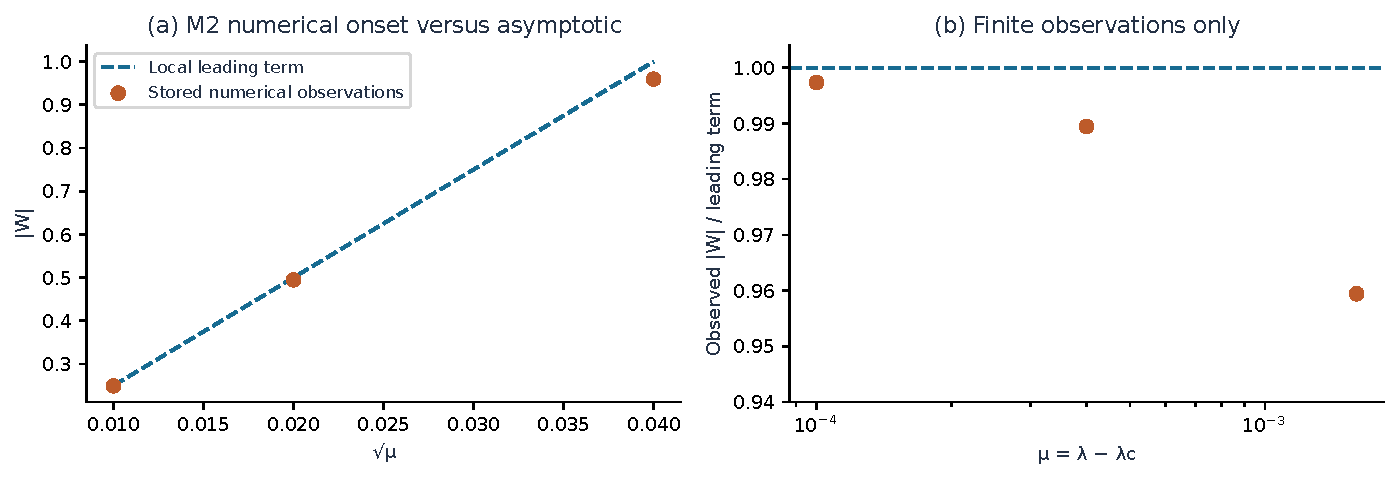
\includegraphics[width=\linewidth]{03_local_onset.pdf}
\caption{Three stored finite numerical observations from the accepted M2 onset table, compared with the leading local asymptotic law \eqref{eq:Wscale}. The original runs used 600000, 150000 and 37500 updates at $\mu=10^{-4},4\cdot10^{-4},1.6\cdot10^{-3}$; they were not rerun for this paper. The line is an asymptotic expression, not certified continuation or an error band. The certified range of that asymptotic approximation is unspecified. These observations do not identify the M3 orbit as the continuation of the local branch.}
\label{fig:onset}\end{figure}

\section{Certified entrance capture at a fixed parameter}
\subsection{The exact model and the trapping box}
Now set $\lambda=\lambda_c+1/200$, where $\lambda_c$ means the exact value in \eqref{eq:critical}, and use
\begin{equation}
 \Om_0=\sqrt3f_1=(1,-1/2-\iu\sqrt3/2,-1/2+\iu\sqrt3/2)^T,
 \qquad\|\Om_0\|^2=3.\label{eq:entranceM3}
\end{equation}
The normalization is part of the theorem. Multiplying the unnormalized Fourier triple by $\sqrt3$ would instead give squared norm nine and is not this entrance. A decimal or binary64 value of $\lambda_c$ is not substituted for the exact parameter.

The closed, five-dimensional box $U_+$ is defined by the rational endpoint strings at
\begin{quote}\small
\path{reproducibility/inputs/m3_accepted_support.json}\\
\texttt{values.exact\_receipts.Up}.
\end{quote}
Each string is an exact integer or numerator/denominator. The same object is regenerated by the portable verifier. Its selected center $c_*$ and weights $r_i>0$ are defined at \texttt{centers} and \texttt{positive\_weights} in that object. They determine the norm $\|z\|_r=\max_i|z_i|/r_i$. Rounded displays are
\begin{align}
 c_*&\simeq(-.06084823646,-.06367959909,-.07761457213,-.01014967245,.43725288805),\nonumber\\
 r&\simeq(3.53225901,3.64418968,4.25148940,1.09846935,10)\,10^{-5}.\label{eq:trapdisplay}
\end{align}
These displays do not redefine the exact endpoints. Because of independent outward endpoint construction, readers should use the receipt rather than reconstructing $U_+$ from rounded $c_*\pm r$.

\begin{theorem}[Fixed-parameter capture, repaired M3]\label{thm:M3}
For \eqref{eq:params} and \eqref{eq:entranceM3} at $\lambda=\lambda_c+1/200$, the exact quotient trajectory is in $\operatorname{int}U_+$ at index $301$. On $U_+$, $\Fh^2$ maps strictly into itself and has Lipschitz constant at most $4789/5000=0.9578$ in $\|\cdot\|_r$. It has a unique fixed point $p$ there, with $\Fh(p)=H(p)\ne p$.

Put $\Om_*^{(+)}=s(p)$ and $\Om_*^{(-)}=F(\Om_*^{(+)})=e^{\iu\theta_p}\overline{\Om_*^{(+)}}$. Then $F(\Om_*^{(-)})=\Om_*^{(+)}$. For some constant $\beta$, with parity anchored at entry,
\begin{equation}
 \Om_{301+2m}\longrightarrow e^{\iu\beta}\Om_*^{(+)},\qquad
 \Om_{302+2m}\longrightarrow e^{\iu\beta}\Om_*^{(-)}.
\label{eq:fulllimit}
\end{equation}
Convergence is geometric per two steps. The limiting $W$ and $\Gamma$ are nonzero and reverse sign at each step. The conjugate entrance $\sqrt3f_2$ satisfies the conjugate conclusion.
\end{theorem}

\subsection{Proof enclosures and direct entry}
The computer-assisted part uses the fixed certified M2 host, interval-derived $V$ and interval-derived $\lambda_c$, with 80 interval digits and 90 point digits. Repeated evaluation over the host enclosure may widen dependencies; it still includes the same exact host and parameter. The original M2 host certificate is recomputed before propagation in the portable replay.

For a convex input box $X$ and selected $c\in X$, the mean-value enclosure is
\begin{equation}
 F(X)\subseteq F(c)+[DF(X)](X-c).\label{eq:meanvalue}
\end{equation}
All 301 propagation centers are checked inside their boxes. The first 21 updates use six real coordinates and full interval phase evaluation. At index 21 the gauge conversion is certified; quotient propagation then reaches $X_{300}$ and performs one further step. The repaired direct entry is
\begin{equation}
 \Fh(X_{300})\subseteq X_{301}\subset\operatorname{int}U_+.\label{eq:entry}
\end{equation}
The enclosure $X_{301}$ occupies less than $0.014584$ of the chosen weighted radius about $c_*$. The theorem uses 301 as a sufficient index, not as a first-entry result.

Let $E_-$ be the computed outer enclosure of $\Fh(U_+)$. The notation is deliberate: $\Fh(U_+)\subseteq E_-$, not equality. Inclusion of $X_{300}$ in $E_-$ would not alone prove capture, because an arbitrary point of an outer image box need not belong to the actual image. The older inference is withdrawn. The interval enclosure of $\Fh(E_-)$ failing to fit inside $U_+$ is likewise not evidence of an actual escaping orbit. Neither issue is used in \eqref{eq:entry}.

\begin{table}[htbp]\centering\small
\begin{tabular}{p{.63\linewidth}r}\toprule
Certified quantity (conservative decimal statement) & Bound\\\midrule
Full pre-sync radii, first 21 updates & $>0.04221$\\
Gauge conversion $|u^T\Om_{21}|^2$ & $>56.90$\\
Quotient pre-sync real parts, through index 300 & $>1.3096$\\
Quotient gauge denominator, same propagation & $>7.7839$\\
Trap pre-sync radii & $>1.5073$\\
Trap pre-sync real parts & $>1.5046$\\
Trap gauge denominator & $>8.8698$\\
Weighted two-step derivative norm & $<0.9578$\\
Smallest strict self-inclusion coordinate margin & $>4.63\cdot10^{-7}$\\
Coordinate-five separation of $U_+$ and $E_-$ & $>0.8743$\\
Krawczyk inverse-defect weighted norm & $<0.1102$\\\bottomrule
\end{tabular}
\caption{Proof margins from the repaired M3 replay, rounded outward to the coarser statements shown. Exact rational endpoints and comparisons are in the supplement. No table entry is a nominal trajectory estimate.}
\label{tab:bounds}\end{table}

\subsection{Contraction and the separate symmetry certificate}
Let $J_1$ enclose $D\Fh(U_+)$ and $J_2$ enclose $D\Fh(E_-)$. Then $J_2J_1$ encloses the derivative of $\Fh^2$ on $U_+$. Interval evaluation of the center image, followed by \eqref{eq:meanvalue}, gives strict self-inclusion. The exact weighted row bounds satisfy
\begin{equation}
 \max_i\frac{\sum_j\sup|(J_2J_1)_{ij}|r_j}{r_i}<\frac{4789}{5000}<1.\label{eq:contraction}
\end{equation}
The compact box is closed and convex and is complete in this norm. The chart bounds in Table \ref{tab:bounds} imply $C^1$ regularity on a neighborhood of the relevant boxes. Applying the mean-value inequality along segments yields the contraction bound, so Banach's fixed-point argument gives a unique $p\in U_+$ \cite{Banach}; the complete-metric-space statement is also Theorem 1.3 of \cite{Kuznetsov}. In particular $\|\Fh^{2m}(z)-p\|_r\le q^m\|z-p\|_r$ for $q=4789/5000$. Disjointness of $E_-$ and $U_+$ excludes period one.

Contraction alone would not identify the quotient cycle as $H$-reflected. Define $R(z)=H\Fh(z)-z$. With a chosen fixed approximate inverse $Y$, the separate Krawczyk box is
\begin{equation}
 K(U_+)=c_*-YR(c_*)+\bigl(I-Y[DR(U_+)]\bigr)(U_+-c_*).
\label{eq:kraw}
\end{equation}
Interval center values and derivatives give $K(U_+)\subset\operatorname{int}U_+$ and weighted defect norm below $0.1102$. This verifies nonsingularity of $Y$ and existence of a zero $z_*$ of $R$ in the box; it is an interval-existence argument, not a conclusion from a tiny nominal residual \cite{Rump}. Since $H$ commutes with $\Fh$, $\Fh(z_*)=Hz_*$ implies $\Fh^2(z_*)=z_*$. Banach uniqueness then gives $z_*=p$.

These steps prove the quotient assertions of Theorem \ref{thm:M3}. The computational inequalities can be rerun without any installed kernel, UI, personal input path or model service. Rounded point data only select $c_*$, weights and $Y$; interval enclosures and exact endpoint comparisons validate those choices.

\begin{figure}[htbp]\centering
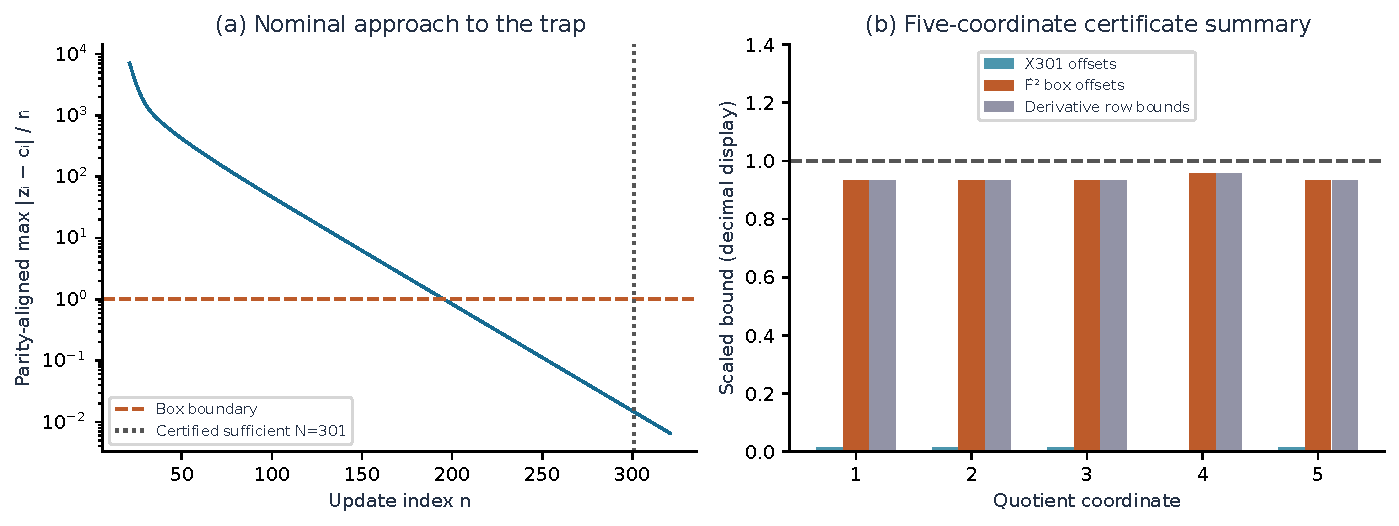
\includegraphics[width=\linewidth]{04_capture.pdf}
\caption{The repaired capture result. Panel (a) is a 130-digit nominal illustration, reflecting the imaginary quotient coordinates on the opposite parity before measuring distance to the selected trap center. It does not prove first entry. Panel (b) displays exact-receipt bounds as rounded bars: entry offsets, two-step image offsets and derivative row bounds are distinct quantities. The five-dimensional rational inequalities, not the plot or a lower-dimensional projection, establish capture and contraction.}
\label{fig:capture}\end{figure}

\subsection{Full-state lift and phase summability}
On the trapped cycle, equivariance and $\Fh(p)=Hp$ imply
\begin{equation}
 F(\Om_*^{(+)})=e^{\iu\theta_p}\overline{\Om_*^{(+)}},\qquad
 F^2(\Om_*^{(+)})=e^{\iu\theta_p}\overline{F(\Om_*^{(+)})}=\Om_*^{(+)}.
\end{equation}
A generic quotient cycle could instead lift to a relative cycle with nonzero total phase. Here the extra $H$-equation removes that ambiguity.

It remains to justify a \emph{single limiting overall rotation} for the approaching full trajectory, not merely quotient convergence. Write $\Om_n=e^{\iu\alpha_n}s(z_n)$ and let $\theta(z)$ be the one-step gauge increment. On the two compact neighborhoods the established positive denominators permit smooth real lifts of these angles. Then
\begin{equation}
 \alpha_{n+2}-\alpha_n=h(z_n),\qquad h(z)=\theta(z)+\theta(\Fh(z)).
\end{equation}
Conjugation gives $h(p)=h(Hp)=0$. Smoothness gives a finite Lipschitz constant for $h$ on the relevant neighborhoods. Quotient contraction therefore bounds the increments on each parity by $Kq^m$. Their tails sum to at most $Kq^m/(1-q)$. Thus $\alpha_{301+2m}\to\beta$ geometrically, while $\alpha_{302+2m}\to\beta+\theta_p$ modulo $2\pi$. Combining this with convergence of $s(z_n)$ proves \eqref{eq:fulllimit}. The raw alternating sequence $\alpha_n$ need not have a single limit; its two parity limits include the intrinsic cycle phase.

Interval evaluation of \eqref{eq:SA}--\eqref{eq:W} over $U_+$ gives, with coarse outward rounding,
\begin{equation}
 1.3342<W_x<1.3352,\quad .8181<W_y<.8190,\quad
 -.01780<\Gamma<-.01645,\quad W_z=0.
\end{equation}
Since $p\in U_+$, these exclude zero at the limiting point. Conjugation makes the other point's values their negatives, and common phase does not affect them. The two-step mean vanishes even though their alternating magnitude persists. Finally $F(\overline\Om)=\overline{F(\Om)}$ carries the entire entrance result to $\sqrt3f_2$; a second trajectory experiment is unnecessary. This completes the proof of Theorem \ref{thm:M3}.

\begin{figure}[htbp]\centering
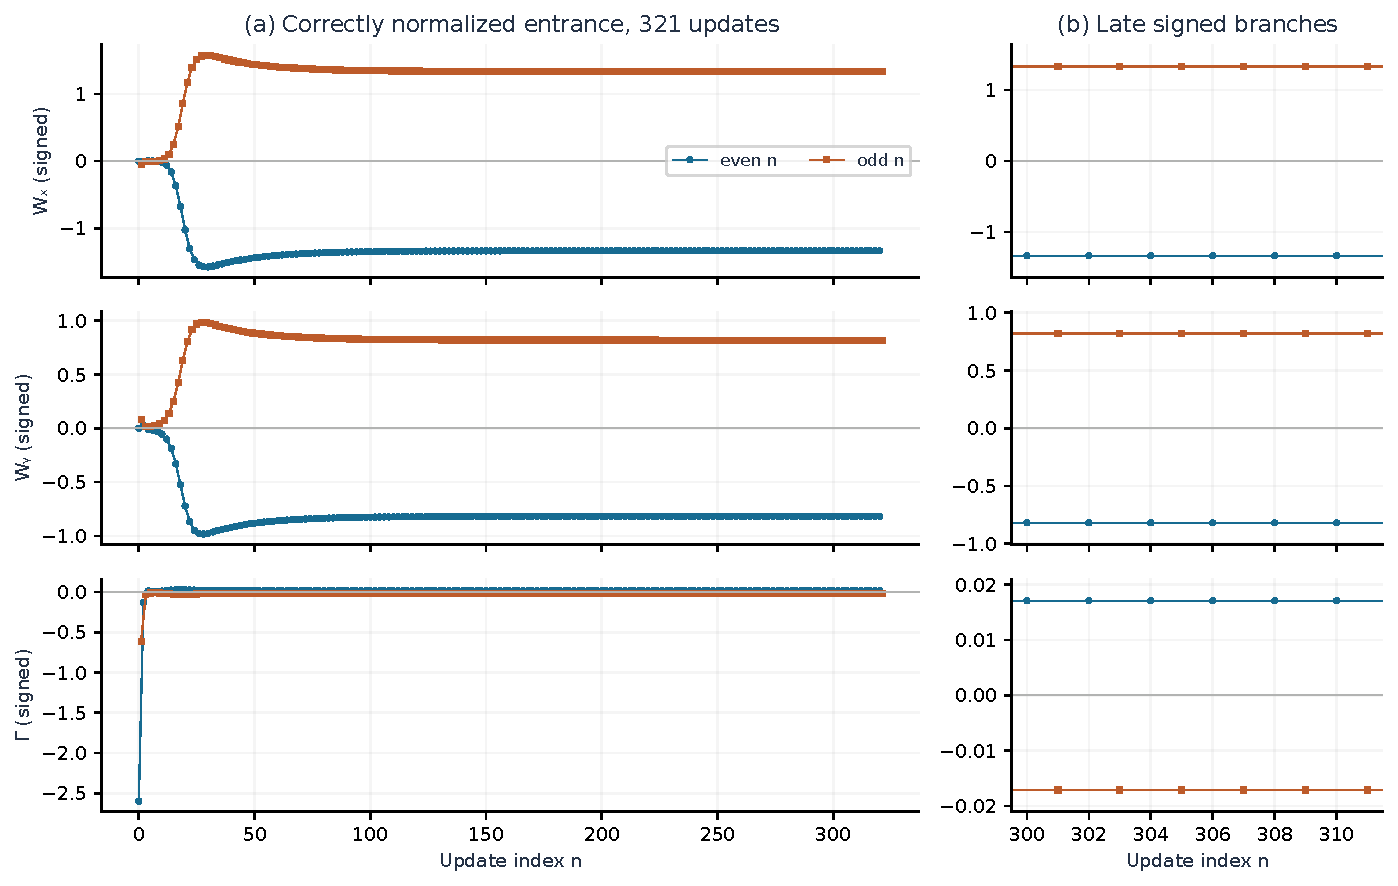
\includegraphics[width=.98\linewidth]{02_signed_trajectory.pdf}
\caption{Signed $W_x,W_y,\Gamma$ for the entrance \eqref{eq:entranceM3} at $\lambda=\lambda_c+1/200$. A bounded 321-update, 130-digit nominal replay was prepared for this figure using the accepted nominal formulation, with its quotient points at 300 and 301 checked inside the accepted exact enclosures. Lines connect equal parity only. The late window shows the reversal hidden by a magnitude-only plot. This numerical illustration is separate from the interval proof and from the differently normalized withdrawn auxiliary symmetry run.}
\label{fig:trajectory}\end{figure}

\section{What the two theorems do and do not establish}
M2 proves existence of a local branch for sufficiently small positive $\mu$. M3 proves capture from one normalized entrance by a specified $H$-symmetric two-cycle at $\mu=1/200$. The continuation of that captured cycle from the M2 branch has not been established. Similar orientation, amplitude or finite-run agreement does not replace continuation. Such a result is not required for either theorem and is not pursued here.

The capture theorem is not a global basin theorem, a first-entry theorem or a claim for all entrance amplitudes. The local coefficient does not supply a universal generation threshold or a guarantee at $\lambda=0.5$. Exact real-arithmetic statements do not automatically hold for the discontinuous binary64 rounding map. Stored rounded parameters, algebraic initial components and runtime implementation identities must remain distinct in any numerical comparison.

The attachment is finite-dimensional and kinematic. It specifies no interpolation over a surface or volume, no magnetic field lines, no cap flux, no charge or current, no calibrated energy and no Maxwell or dynamo law. No additional physical premise is required for the mathematical results proved here. Physical identification would need new assumptions and evidence. No such assumptions are adopted in this manuscript.

Paper F's small-seed angular law transfers to $W$ through the orientation-preserving similarity $T|_{e^\perp}$ with its fixed angular offset, subject to Paper F's own equal-coefficient, local and nonzero-direction hypotheses. It does not imply sustained circulation or six-axis attraction here. Likewise, M1's separate ring analysis and S01 sideband result are not needed for the triad certificate. The exact residue-three lift remains in its invariant sector; a transverse instability does not make an exactly lifted state leave it without a perturbation. No ring robustness or M4 problem is opened. The optional X01 state-dependent connection is unadopted and absent from all proofs and software designs here.

\section{Reproducibility and observation design}
The supplement contains the controlling joint records and final corrections, immutable accepted inputs, the original M2 and repaired M3 verifier sources, and an explicitly labelled publication I/O wrapper. It first recomputes the integer-interval M2 certificate, then recomputes the M3 propagation, trapping, derivative and symmetry enclosures. Exact endpoint checks establish the public contraction bound and nonzero observables. A separate nominal replay tests consistency with the two entry enclosures; it is not an independent interval engine. The present replay passed 28 M3 verdicts and 23 supporting predicates. These counts include bookkeeping checks and are not counts of independent theorems.

The M2 onset figure reuses three rows of the original finite-run table; no long onset trajectories were rerun. The other nominal figure data come from the declared short replay. All four figures have deterministic scripts, data and source identities. Source manifests authenticate bytes; the running verifiers, mathematical arguments and reviewed rounding operations establish the proof, not hashes by themselves.

The companion \path{OBSERVATION_IMPLEMENTATION_CONTRACT.md} is a design for passive current-model application features. It specifies one pure mathematical owner, additive public facade functions, existing isolated-worker dispatch and immutable derived caches. It separates stored-state recomputation, one-step accounting prediction and comparison with a genuinely adjacent stored sample. The UI would display signed histories and source terms without becoming a trajectory owner. A static M3 proof card would describe the accepted exact-model result; new floating runs would not inherit it. Implementation, packaging certification and publication are separate future authorizations. No kernel or UI changes accompany this draft.

\section{Conclusion}
Within the stated real-linear equivariant class, $W=TC$ is the geometry-attached planar axial observable, while $\Gamma=e^TC$ retains the complementary hidden channel area. For the accepted Fourier entrance, unequal $k$ exposes that area in $W$ after one exact update, provided the entrance amplitude, $\epsilon$ and all factors $b_i$ are nonzero. This conversion and the finite-step accounting are algebraic statements, not claims of a physical field.

For the specified unequal-$k$ host, the positive interval-certified cubic coefficient establishes a local supercritical flip for sufficiently small positive $\mu$. Separately, at the exact $\lambda=\lambda_c+1/200$, the entrance with squared norm three is certified to enter the repaired M3 trap at $N=301$ and converge, up to one constant common-phase rotation, to a nonzero $H$-symmetric complex two-cycle. Its $W$ and $\Gamma$ alternate in sign. The local M2 branch and the fixed-parameter M3 orbit have not been proved to form one continued branch. No physical magnetic field has been identified.

\appendix
\section{Replay entry points and exact objects}
From the paper directory, with Python 3.11 and \texttt{mpmath==1.3.0}, run
\begin{quote}\small
\texttt{python -I -B reproducibility/replay.py --output <new-external-directory>}
\end{quote}
The output directory must be new. The process writes copies and results there, leaving the supplement and original evidence intact. It needs no repository package import, database, network or service. The recomputed M2 \texttt{integer\_interval\_certificate} must equal its accepted input, and the M3 exact $U_+$, weights and $X_{301}$ are compared to the accepted receipt after actual recomputation.

The exact trap and weights reside in \texttt{m3\_accepted\_support.json} under \texttt{values.exact\_receipts}; \texttt{Um} is the historical source key for $E_-$, \texttt{qbox} for $X_{300}$, \texttt{q301} for $X_{301}$, \texttt{Zw} for the two-step image enclosure, and \texttt{Kr} for the symmetry-equation Krawczyk image. The original source keys are retained for byte provenance, while the manuscript uses corrected set notation. The M2 certificate expresses interval endpoints as integers divided by $2^{240}$; these are not display strings.

The portable wrapper preserves the original mathematical verifier bodies. Its adapted supporting script changes paths and replaces historical multi-precision-log comparisons with exact accepted-object comparisons. Adaptations and source hashes are documented separately. The 80-digit replay is new publication-preparation execution, not a claim to reproduce all original hardware or every historical precision run.

\section{Evidence provenance and review boundary}
The local review package identifies repository baseline \nolinkurl{64ddea159e0e69888926aa21fa281e42f5dd50b4}. The accepted M1 common core has SHA-256
\begin{quote}\small\nolinkurl{a14e5a108dc49c6f0c75950747567132993bd47b2d12ff7ee69d689a52768ef6}.\end{quote}
M2's later sign certificate and the corrected odd remainder and two-step multiplier supersede the original report's numerical-only sign status and multiplier wording. M3's final acceptance includes the repaired index-301 proof and withdrawal of branch identification. Older reports and raw result labels remain archival evidence, not competing final statements. The supplementary claim map makes these corrections explicit.

This manuscript was prepared with AI-assisted synthesis and computational checking from the accepted local records. Their internal cross-review is not external peer review. All included local evidence copies retain their attribution and hashes. Publication and redistribution approval remains to be decided for this assembled package; the repository's Apache-2.0 software license does not automatically license papers, figures or research datasets. No external full-text PDFs or figures are redistributed here.

\begin{thebibliography}{99}\small
\item[] Repository paths in references [1]--[5] identify the cited editions at baseline \nolinkurl{64ddea159e0e69888926aa21fa281e42f5dd50b4}; see Appendix B and the project-source manifest. Supplement paths in [6]--[8] are relative to this Paper G edition.
\bibitem{PA} H. F. Halldórsson, \emph{Cycle-Covering Dynamics of a Three-State Nonlinear Kernel}, Paper A v1.0 (21 September 2026), especially \S6.1. \path{papers/PAPER_A/publication/paper_A_publication.md}.
\bibitem{PB} H. F. Halldórsson, \emph{Triadic Chirality and Orientation Geometry}, Paper B v0.1.2, frames and transported areas. \path{papers/PAPER_B/publication/v0.1.2/}.
\bibitem{PE} H. F. Halldórsson, \emph{The Tri-Octagon Z Manifold: Harmonic Macro Geometry, Chiral Deformation, and Diagnostic Dynamics}, Paper E v0.1.1. \path{papers/PAPER_E/v0.1.1/PAPER_E_Z_MANIFOLD_v0.1.1.md}.
\bibitem{PF} H. F. Halldórsson, \emph{Transverse Chirality, Dihedral Harmonic Selection, and Local Linearization in a Three-Channel Nonlinear Map}, Paper F v0.2. \path{papers/PAPER_F/PAPER_F_PUBLICATION_v0.2.md}.
\bibitem{Atlas} \emph{TRIOCTAGON Mathematical Atlas 08: Boundary Response, Fixed SRG, Initialization Handoff}, v0.1, 29 September 2026, local source packet, especially the Fourier-form endpoint; no physical boundary law. Repository \path{research/mathematical_atlas/entry_08_boundary_srg_handoff/}.
\bibitem{M1} \emph{M1 Joint Acceptance Record v0.2} and \emph{Common Equations Candidate v0.2}, accepted CE01--CE11 with stated domains; final assents supersede the candidate-status label. The separate S01 sideband proof is in the GPT reconciliation note, \S4, retained as \path{reproducibility/authorities/M1_RECONCILIATION_AND_S01.md} with its final disposition in the joint record. Supplement \path{reproducibility/authorities/}.
\bibitem{M2} \emph{M2 Joint Acceptance Record v0.1}, with GPT's analytic interval sign certificate, Claude's correction addendum and Codex's acceptance addendum, 1--2 October 2026. Supplement \path{reproducibility/authorities/M2_JOINT_ACCEPTANCE.md}, \path{reproducibility/authorities/M2_CLAUDE_CORRECTIONS.md}, \path{reproducibility/authorities/M2_CODEX_ASSENT.md}; input \path{reproducibility/inputs/m2_accepted_certificate.json}.
\bibitem{M3} \emph{M3 Joint Acceptance Record v0.1}, Claude repaired review v0.2 and Codex reconciliation addendum v0.1, 4 October 2026. Supplement \path{reproducibility/authorities/M3_JOINT_ACCEPTANCE.md}, \path{reproducibility/authorities/M3_CLAUDE_REPAIRED_REVIEW.md}, \path{reproducibility/authorities/M3_CODEX_RECONCILIATION.md}.
\bibitem{Kuznetsov} Y. A. Kuznetsov, \emph{Elements of Applied Bifurcation Theory}, 2nd ed., Springer-Verlag, New York, 1998, \S\S4.4--4.5 (Theorems 4.3--4.4), 5.1--5.2 and 5.4.2. \url{https://doi.org/10.1007/b98848}. Access copy: \url{https://wwwf.imperial.ac.uk/~dturaev/kuznetsov.pdf}. Standard flip and center-manifold results; no new attribution to this paper.
\bibitem{Banach} S. Banach, Sur les opérations dans les ensembles abstraits et leur application aux équations intégrales, \emph{Fundamenta Mathematicae} 3 (1922), 133--181. \url{https://doi.org/10.4064/fm-3-1-133-181}. Contraction principle; its iteration estimate is applied explicitly above.
\bibitem{Rump} S. M. Rump and S. Graillat, Verified error bounds for multiple roots of systems of nonlinear equations, \emph{Numerical Algorithms} 54(3) (2010), 359--377. \url{https://doi.org/10.1007/s11075-009-9339-3}. Theorem 2.1 (simple-root interval inclusion). Author-hosted text: \url{https://www.tuhh.de/ti3/paper/rump/RuGr09.pdf}. The multiple-root results are not used.
\end{thebibliography}
\end{document}
